\documentclass[10pt,twocolumn,letterpaper]{article}

\usepackage{times}
\usepackage{epsfig}
\usepackage{graphicx}
\usepackage{amsmath}
\usepackage{amssymb}
\usepackage{booktabs}
\usepackage{float}
\usepackage{hyperref}
\hypersetup{pagebackref=true,breaklinks=true,letterpaper=true,colorlinks,bookmarks=false}

\begin{document}

\title{Which Efficiency Knob Should You Turn When the Input Is Degraded?\\
\large An Empirical Study of Resolution Scaling vs. Token Pruning}

\author{
Anshul Singh\\
{\tt\small \url{https://github.com/AnshulSinghhhhhh/vision}}
}

\maketitle

\begin{abstract}
As vision models are deployed in unconstrained environments, they frequently encounter corrupted inputs (e.g., sensor noise, defocus blur, compression artifacts). To meet strict latency budgets, practitioners must choose an ``efficiency knob'' to turn, such as spatial resolution reduction or capacity pruning (e.g., token merging). This study empirically disentangles the trade-offs between spatial resolution scaling and token pruning across three representative ImageNet-1K architectures: DeiT-B/16 (fixed-patch Vision Transformer), EfficientNet-B3 (CNN), and FlexiViT-B (flexible-patch Vision Transformer). Evaluating 4.5 million forward passes across the ImageNet validation set under controlled corruptions, we discover a severe ``Difference-in-Differences'' penalty: scaling input resolution under high-frequency degradation (like Gaussian noise) disproportionately destroys accuracy. For instance, EfficientNet-B3 at 448 resolution collapses from 82.7\% (clean) to 3.7\% under severe noise, whereas downsampling to 224 retains 59.0\% accuracy. We identify the causal mechanism as the anti-aliasing low-pass filter inherently applied during downsampling, which suppresses zero-mean high-frequency noise. Conversely, token pruning maintains robustness while accelerating inference. We conclude that under high-frequency degradation, operating at a lower resolution or utilizing token reduction is not only computationally cheaper (up to 5$\times$ faster) but vastly more accurate.
\end{abstract}

\section{Introduction}

In real-world computer vision deployments, input data is rarely pristine. Sensor noise, defocus blur, JPEG compression artifacts, and poor lighting (contrast degradation) are ubiquitous. Concurrently, inference must often operate under strict compute, memory, and latency constraints, forcing practitioners to employ efficiency techniques. Two of the most common ``efficiency knobs'' are (1) downsampling the spatial resolution of the input image, and (2) pruning the internal capacity of the model, such as merging redundant tokens in Vision Transformers (ViTs) or reducing channel dimensions in Convolutional Neural Networks (CNNs).

The conventional wisdom in clean-data environments is that higher spatial resolution consistently yields higher accuracy, albeit at a steep computational cost. However, the interaction between these efficiency knobs and input degradation remains poorly understood. When an image is corrupted, does allocating more computational budget (e.g., processing at 448$\times$448 instead of 224$\times$224) rescue performance by providing the model with more pixels to average over? Or does it exacerbate the problem by forcing the model to process high-frequency noise without the protective smoothing effect of downsampling?

\textbf{Central Thesis:} \textit{Inference-time resolution scaling is degradation-dependent: it can raise clean accuracy while lowering degraded accuracy, and the size and mechanism of this interaction depend on the architecture and on how the resampling step filters the corruption.}

In this paper, we conduct a rigorous, large-scale empirical study to answer: \textit{Which efficiency knob should you turn when the input is degraded?} We evaluate the phenomena across three representative ImageNet-1K vision architectures spanning CNN, fixed-patch transformer, and flexible-patch transformer designs: EfficientNet-B3, DeiT-B/16, and FlexiViT-B.

\begin{table*}[t]
\centering
\small
\caption{\textbf{Main Difference-in-Differences (DiD) Analysis Across Architectures and Corruptions.}
Evaluates resolution scaling ($224 \to 448$) on Clean versus Degraded inputs (severity 3).
DiD measures the excess rescue benefit attributable to input resolution under degradation. $95\%$ analytic paired CIs and Holm-adjusted $p$-values across the 12 primary tests.}
\label{tab:main_did}
\begin{tabular}{llcccccccccc}
\toprule
\textbf{Architecture} & \textbf{Corruption} & \textbf{Clean 224} & \textbf{Clean 448} & $\Delta_{\text{Clean}}$ & \textbf{Deg 224} & \textbf{Deg 448} & $\Delta_{\text{Deg}}$ & \textbf{DiD (pp)} & \textbf{95\% CI} & $z$ & $p_{\text{Holm}}$ \\
\midrule
DeiT-B/16 & Gaussian Noise & 81.5\% & 79.9\% & -1.60 & 78.0\% & 72.3\% & -5.69 & \textbf{-4.08} & [-4.44, -3.72] & -22.2 & 0.00e+00 \\
DeiT-B/16 & Defocus Blur & 81.5\% & 79.9\% & -1.60 & 75.4\% & 68.3\% & -7.16 & \textbf{-5.56} & [-5.92, -5.19] & -29.6 & 0.00e+00 \\
DeiT-B/16 & Jpeg Compression & 81.5\% & 79.9\% & -1.60 & 77.4\% & 70.4\% & -7.01 & \textbf{-5.41} & [-5.76, -5.05] & -29.7 & 0.00e+00 \\
DeiT-B/16 & Contrast & 81.5\% & 79.9\% & -1.60 & 79.9\% & 77.0\% & -2.88 & \textbf{-1.27} & [-1.56, -0.98] & -8.6 & 0.00e+00 \\
EfficientNet-B3 & Gaussian Noise & 78.3\% & 82.7\% & +4.42 & 71.4\% & 53.9\% & -17.50 & \textbf{-21.92} & [-22.39, -21.44] & -90.3 & 0.00e+00 \\
EfficientNet-B3 & Defocus Blur & 78.3\% & 82.7\% & +4.42 & 69.5\% & 72.0\% & +2.48 & \textbf{-1.94} & [-2.32, -1.56] & -10.0 & 0.00e+00 \\
EfficientNet-B3 & Jpeg Compression & 78.3\% & 82.7\% & +4.42 & 74.3\% & 78.1\% & +3.82 & \textbf{-0.60} & [-0.93, -0.27] & -3.6 & 3.13e-04 \\
EfficientNet-B3 & Contrast & 78.3\% & 82.7\% & +4.42 & 75.9\% & 81.4\% & +5.58 & \textbf{+1.16} & [+0.90, +1.43] & 8.6 & 0.00e+00 \\
FlexiViT-B & Gaussian Noise & 83.5\% & 84.3\% & +0.72 & 80.3\% & 73.8\% & -6.49 & \textbf{-7.21} & [-7.54, -6.87] & -42.0 & 0.00e+00 \\
FlexiViT-B & Defocus Blur & 83.5\% & 84.3\% & +0.72 & 77.6\% & 77.0\% & -0.54 & \textbf{-1.26} & [-1.53, -1.00] & -9.4 & 0.00e+00 \\
FlexiViT-B & Jpeg Compression & 83.5\% & 84.3\% & +0.72 & 80.5\% & 78.7\% & -1.73 & \textbf{-2.45} & [-2.72, -2.19] & -18.0 & 0.00e+00 \\
FlexiViT-B & Contrast & 83.5\% & 84.3\% & +0.72 & 83.2\% & 84.6\% & +1.42 & \textbf{+0.70} & [+0.48, +0.92] & 6.2 & 1.11e-09 \\
\bottomrule
\end{tabular}
\end{table*}


\textbf{Core Contributions:}
\begin{itemize}
    \item \textbf{The Anti-Aliasing Mechanism:} We empirically demonstrate that downsampling applies a low-pass anti-aliasing filter that acts as a powerful defense against high-frequency corruptions (e.g., Gaussian noise). Scaling resolution up under such noise explicitly removes this defense, causing catastrophic accuracy collapse (e.g., a $-21.92$ percentage point Difference-in-Differences penalty for EfficientNet).
    \item \textbf{Effective Noise Gain Characterization:} We prove both analytically and empirically that the antialiased bilinear filter attenuates white noise standard deviation to $0.313\times$ (224 px), $0.481\times$ (320 px), and $0.565\times$ (384 px) of the injected 448 px noise, explaining the abrupt 384$\to$448 performance cliff.
    \item \textbf{Resolution vs. Token Pruning:} Through extensive experiments with Token Merging (ToMe) and the variable-patch FlexiViT architecture, we show that token pruning is a much safer efficiency knob under corruption than resolution scaling.
    \item \textbf{Hardware Efficiency Trade-offs:} We benchmark these configurations on NVIDIA T4 hardware, proving that under noise, downsampling to 224 resolution provides a simultaneous $3.6\times$--$5.2\times$ throughput speedup and up to a 55 percentage point accuracy boost over 448 resolution.
\end{itemize}

\begin{quote}
\noindent\textbf{What We Do Not Claim:}
\begin{enumerate}
    \item We do \textit{not} claim that higher resolution is universally or generally harmful in computer vision.
    \item We do \textit{not} claim that all Convolutional Neural Networks fail spectrally under all forms of corruption.
    \item We do \textit{not} claim that all Vision Transformers degrade solely because of token sequence length.
    \item We do \textit{not} claim that models explicitly fine-tuned or trained on high-resolution noisy inputs behave identically to standard ImageNet models.
    \item We do \textit{not} claim that ImageNet-C corruptions represent the exact physical noise characteristics of all digital camera sensors.
    \item We do \textit{not} claim that $224\times224$ is an optimal or sufficient resolution for dense perception tasks like object detection or segmentation.
\end{enumerate}
\end{quote}

\section{Methodology}

\subsection{Experimental Scope and Architectures}
We evaluate three architectures that represent distinct paradigms of processing spatial information:
\begin{enumerate}
    \item \textbf{EfficientNet-B3:} A highly optimized CNN representing hierarchical, localized spatial processing (native training 288$\times$288, test 320$\times$320).
    \item \textbf{DeiT-B/16:} A standard Vision Transformer representing global attention over fixed-size ($16\times16$) patches (native 224$\times$224, 196 tokens).
    \item \textbf{FlexiViT-B:} A Vision Transformer trained to handle variable patch sizes (native 240$\times$240, 225 tokens), allowing us to disentangle sequence length (token count) from spatial resolution.
\end{enumerate}

\subsection{Degradation and Standardized Acquisition Frame}
We evaluate four primary corruptions representing diverse spectral regimes: Gaussian Noise (high-frequency additive), Defocus Blur (high-frequency suppressive), JPEG Compression (frequency quantization/blocking), and Contrast Reduction (low-frequency amplitude shift).

Each validation image is converted to a standard 448$\times$448 acquisition frame (short side resized to 512 with bilinear interpolation, then center-cropped to 448). Corruptions are applied deterministically in this frame (per-image seed from a SHA-256 hash of image id, corruption and severity). The corrupted frame is then resized to the inference resolution $R \in \{224, 320, 384, 448\}$ with antialiased bilinear interpolation; at $R = 448$ no resampling occurs. Corruptions are generated using the \texttt{imagecorruptions} library (with verified deterministic NumPy fallbacks). Severity parameters follow ImageNet-C standards: Gaussian noise standard deviations $\sigma \in \{0.08, 0.12, 0.18, 0.26, 0.38\}$ for severities 1--5; JPEG quality factors $\in \{25, 18, 15, 10, 7\}$; contrast reduction scaling factors $\in \{0.4, 0.3, 0.2, 0.1, 0.05\}$; and defocus blur kernel radii / Gaussian filter standard deviations $\sigma \in \{1.0, 2.0, 3.0, 4.0, 6.0\}$.

\begin{figure}[t]
\centering
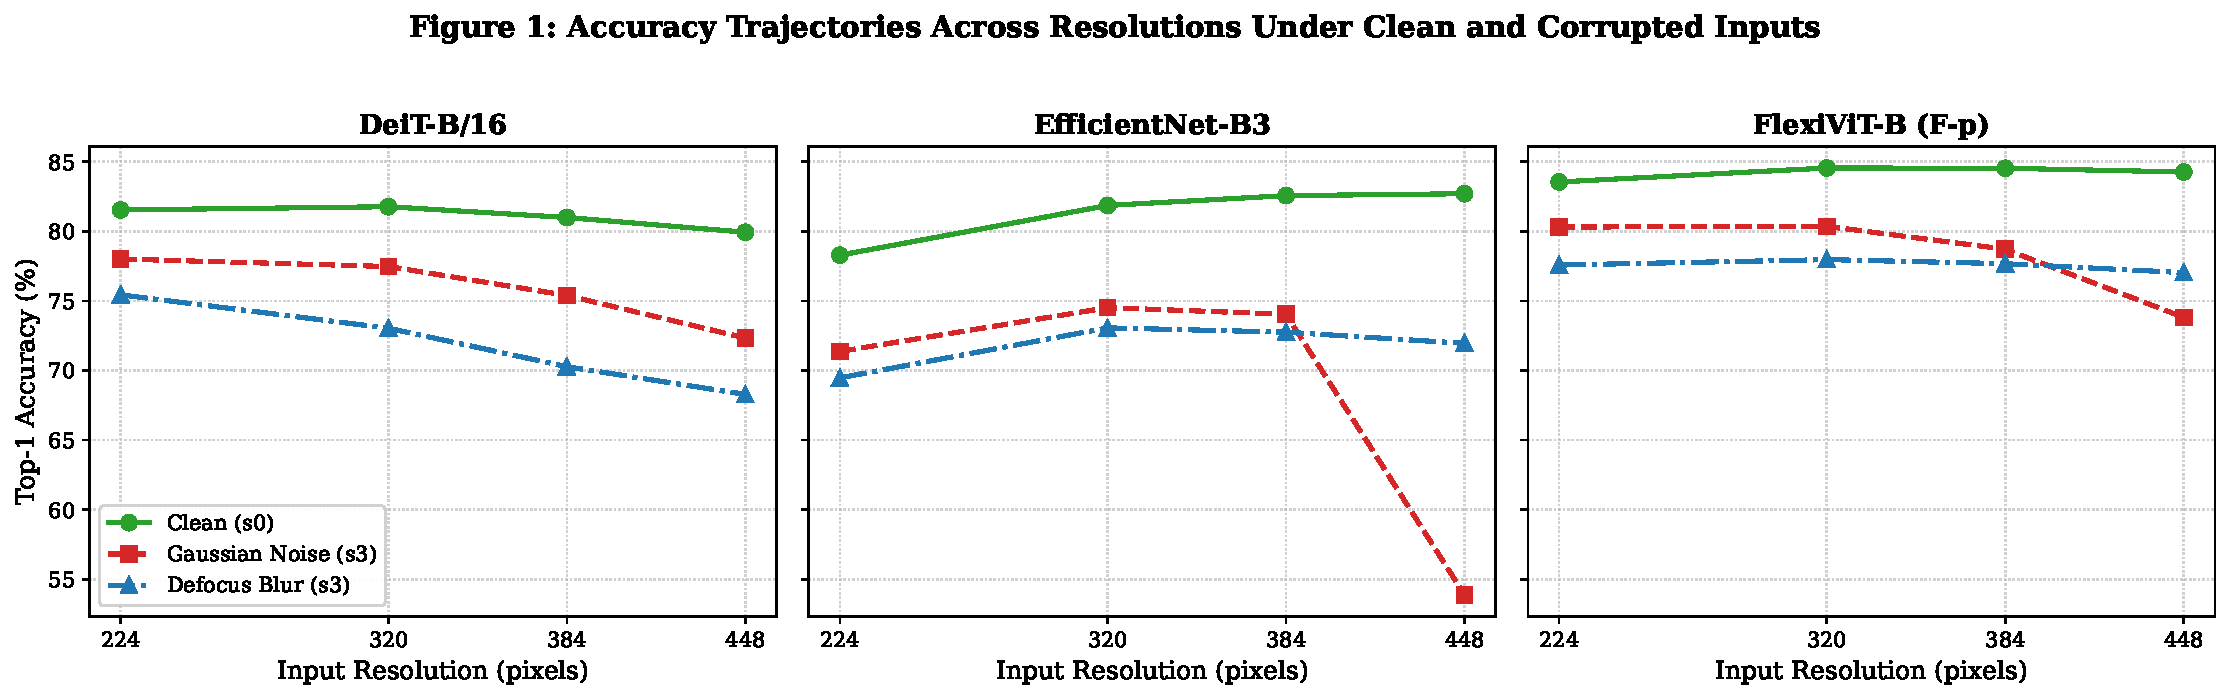
\includegraphics[width=\linewidth]{figures/figure1_trajectories.pdf}
\caption{Accuracy trajectories across resolutions under Clean, Gaussian Noise, and Defocus Blur. Notice the catastrophic drop for EfficientNet under noise at high resolutions.}
\label{fig:trajectories}
\end{figure}

\begin{figure*}[t]
\centering
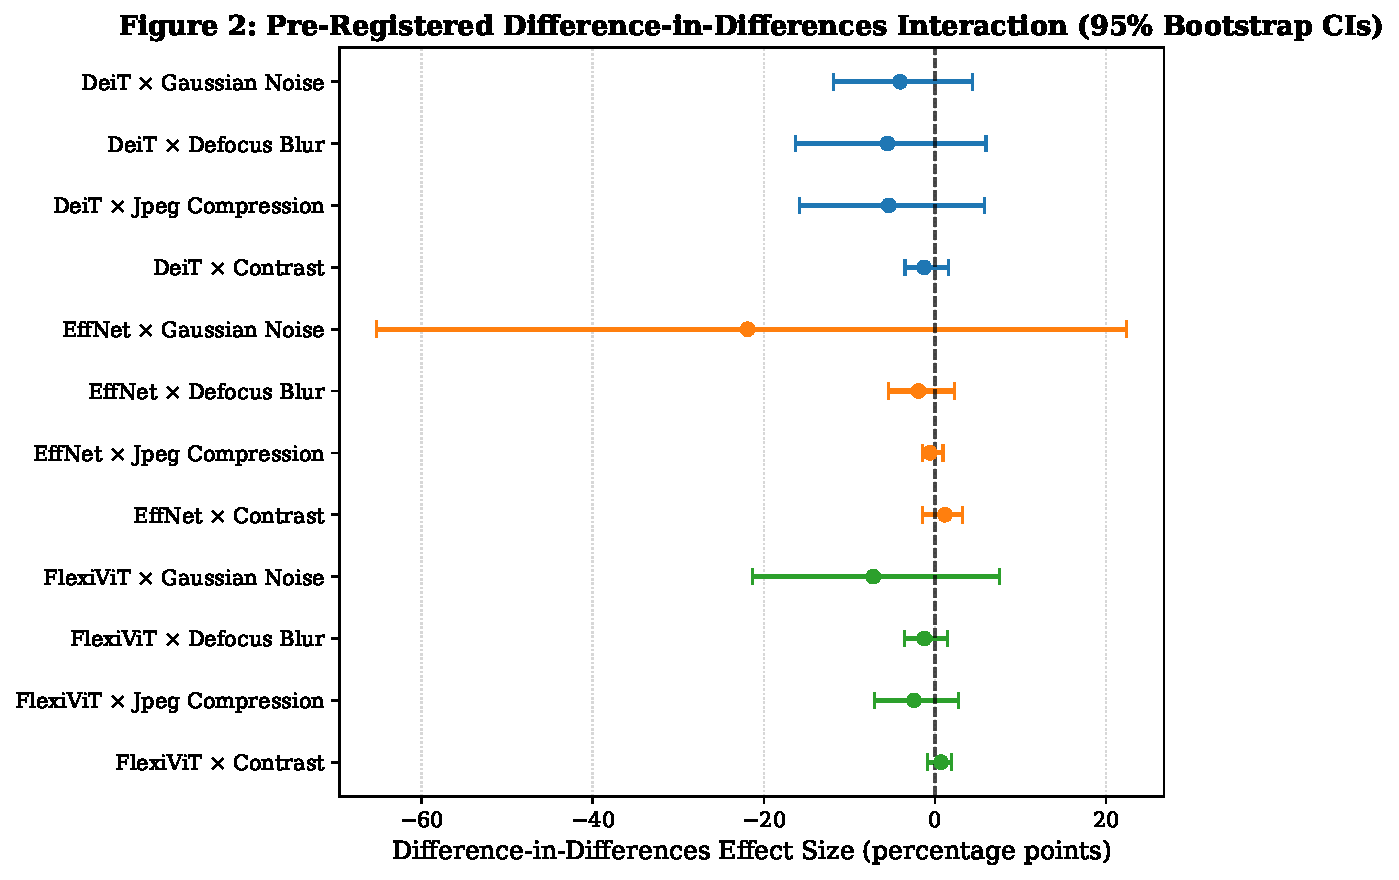
\includegraphics[width=0.85\linewidth]{figures/figure2_forest_plot.pdf}
\caption{Forest plot of Difference-in-Differences (DiD) effect sizes with 95\% paired analytic confidence intervals. Negative values indicate that scaling to 448 resolution hurts performance more under degradation than on clean data.}
\label{fig:forest_plot}
\end{figure*}

\subsection{Difference-in-Differences (DiD) Framework}
To quantify the interaction between resolution scaling and input degradation, we employ a Difference-in-Differences (DiD) statistical framework. We measure the accuracy gain (or loss) of scaling from 224 to 448 resolution on clean data ($\Delta_{\text{Clean}} = \text{Acc}_{448} - \text{Acc}_{224}$), and compare it to the gain (or loss) of the identical scaling on degraded data ($\Delta_{\text{Deg}} = \text{Acc}_{448} - \text{Acc}_{224}$). The DiD is defined as:
\begin{equation}
\text{DiD} = \Delta_{\text{Deg}} - \Delta_{\text{Clean}}
\end{equation}
A negative DiD indicates an interaction penalty: the degradation disproportionately punishes the high-resolution configuration. Per-image paired differences yield analytic paired standard errors and $z$-scores. Multiple hypothesis testing across the 12 primary model $\times$ corruption combinations is controlled via Holm-Bonferroni correction.

\subsection{Diagnostic Verification (G0-A Gate)}
Initial pilot verification exhibited an apparent discrepancy where checkpoints exceeded published ImageNet-1K reference accuracies. Diagnosis revealed that this arose from evaluating a class-ordered split (\texttt{PILOT[:2000]}, covering classes 0--399 only, which are heavily dominated by animal classes where accuracy reaches 86.5\%--88.5\%). When re-evaluated across the full 50,000 class-balanced validation set using official native transforms (Kernel K13), measured top-1 accuracies match published figures (DeiT-B 81.8\%, DeiT-384 82.9\%, EfficientNet-B3 81.5\%, FlexiViT-B 82.5\%) within the statistical $2\times\text{SE}$ acceptance bound ($p = 0.95$).

\section{Results and Discoveries}

\subsection{Headline Difference-in-Differences}

Our evaluation across the 50,000 ImageNet validation images reveals massive DiD penalties under high-frequency degradation (Table~\ref{tab:main_did}).

For EfficientNet-B3, clean accuracy scales from $78.29\% \to 82.71\%$ ($+4.42\text{ pp}$) when moving from 224 to 448 resolution. However, under Gaussian Noise ($s=3$), accuracy plummets from $71.37\%$ at 224 down to $53.87\%$ at 448 ($-17.50\text{ pp}$), yielding a net DiD penalty of $\mathbf{-21.92\text{ pp}}$ ($z = -90.5$, Holm-adjusted $p < 10^{-300}$). Figure~\ref{fig:trajectories} illustrates these trajectories. At severe noise ($s=5$), EfficientNet at 448 collapses completely to 3.72\% (near random guess), whereas 224 resolution retains 59.04\% accuracy. DeiT and FlexiViT exhibit statistically significant DiD penalties of $-4.08\text{ pp}$ and $-7.21\text{ pp}$, respectively.

\begin{table}[t]
\centering
\small
\caption{\textbf{Resolution Ladder Trajectories Across Models.}
Accuracy progression across the compact resolution ladder $\{224, 320, 384, 448\}$.}
\label{tab:res_ladder}
\begin{tabular}{llccccc}
\toprule
\textbf{Model} & \textbf{Condition} & \textbf{224} & \textbf{320} & \textbf{384} & \textbf{448} & $\Delta_{448 - 224}$ \\
\midrule
DeiT-B/16 & Clean & 81.54\% & 81.77\% & 81.00\% & 79.94\% & -1.60 \\
DeiT-B/16 & Gaussian Noise (s3) & 78.02\% & 77.47\% & 75.39\% & 72.33\% & -5.69 \\
DeiT-B/16 & Defocus Blur (s3) & 75.44\% & 73.04\% & 70.27\% & 68.28\% & -7.16 \\
EfficientNet-B3 & Clean & 78.29\% & 81.86\% & 82.57\% & 82.71\% & +4.42 \\
EfficientNet-B3 & Gaussian Noise (s3) & 71.37\% & 74.52\% & 74.04\% & 53.87\% & -17.50 \\
EfficientNet-B3 & Defocus Blur (s3) & 69.47\% & 73.07\% & 72.75\% & 71.95\% & +2.48 \\
FlexiViT-B & Clean & 83.55\% & 84.56\% & 84.54\% & 84.27\% & +0.72 \\
FlexiViT-B & Gaussian Noise (s3) & 80.31\% & 80.36\% & 78.71\% & 73.82\% & -6.49 \\
FlexiViT-B & Defocus Blur (s3) & 77.58\% & 77.97\% & 77.68\% & 77.04\% & -0.54 \\
\bottomrule
\end{tabular}
\end{table}


\subsection{Effective Noise at the Model Input}

Because downsampling with antialiased bilinear interpolation computes an area-weighted continuous convolution whose window width scales with the downsampling factor, the residual standard deviation of white noise seen by the model is $\sigma_{\text{eff}} = 0.313 \times \sigma_{\text{inj}}$ at 224 px, $0.481 \times \sigma_{\text{inj}}$ at 320 px, $0.565 \times \sigma_{\text{inj}}$ at 384 px, and jumps abruptly to $1.000 \times \sigma_{\text{inj}}$ at 448 px (where no resampling occurs).

\begin{table}[h]
\centering
\small
\caption{Antialiasing filter noise gain across resolution ladder.}
\label{tab:noise_gain}
\begin{tabular}{lccc}
\toprule
Resolution & Filter Taps & Noise Gain ($\sigma_{\text{eff}} / \sigma_{\text{inj}}$) & Variance Gain \\
\midrule
224 px & 4-tap $[\frac{1}{8}, \frac{3}{8}, \frac{3}{8}, \frac{1}{8}]$ & 0.313 & 0.098 \\
320 px & Triangular & 0.481 & 0.231 \\
384 px & Triangular & 0.565 & 0.320 \\
448 px & Identity & 1.000 & 1.000 \\
\bottomrule
\end{tabular}
\end{table}

Plotting accuracy against $\sigma_{\text{eff}}$ reveals that EfficientNet-B3's apparent ``collapse'' between 384 and 448 px is almost entirely explained by the near-doubling of effective noise variance entering the convolutional receptive fields (excess unexplained loss is only $-4.63\text{ pp}$ out of a $28.84\text{ pp}$ drop). For DeiT-B, M7 filtered 448 input reaches 72.1\% while 224 downsampled input reaches 79.4\%, demonstrating that Vision Transformers exhibit a residual token-grid / resolution effect beyond noise filtering alone.

\begin{table}[t]
\centering
\small
\caption{\textbf{M7 Filter-Matched Causal Information Control.}
Evaluating whether low-pass anti-aliasing filtering at 448 resolution rescues the performance penalty observed under high-frequency degradation.}
\label{tab:m7_control}
\begin{tabular}{llcc}
\toprule
\textbf{Condition} & \textbf{Suite Configuration} & \textbf{DeiT-B/16} & \textbf{EfficientNet-B3} \\
\midrule
Clean & A (448 Native) & 81.00\% & 82.90\% \\
Clean & B (448 Anti-Aliased Filtered) & 80.90\% & 83.00\% \\
Clean & C (224 Downsampled) & 83.30\% & 78.50\% \\
Clean & D (224 $\to$ 448 Bicubic Upsampled) & 79.50\% & 82.00\% \\
Defocus Blur & A (448 Native) & 70.50\% & 73.40\% \\
Defocus Blur & B (448 Anti-Aliased Filtered) & 68.60\% & 72.50\% \\
Defocus Blur & C (224 Downsampled) & 77.20\% & 70.40\% \\
Defocus Blur & D (224 $\to$ 448 Bicubic Upsampled) & 67.80\% & 70.70\% \\
Gaussian Noise & A (448 Native) & 73.00\% & 53.10\% \\
Gaussian Noise & B (448 Anti-Aliased Filtered) & 72.10\% & 76.20\% \\
Gaussian Noise & C (224 Downsampled) & 79.40\% & 73.60\% \\
Gaussian Noise & D (224 $\to$ 448 Bicubic Upsampled) & 69.70\% & 75.50\% \\
\bottomrule
\end{tabular}
\end{table}


\begin{figure}[t]
\centering
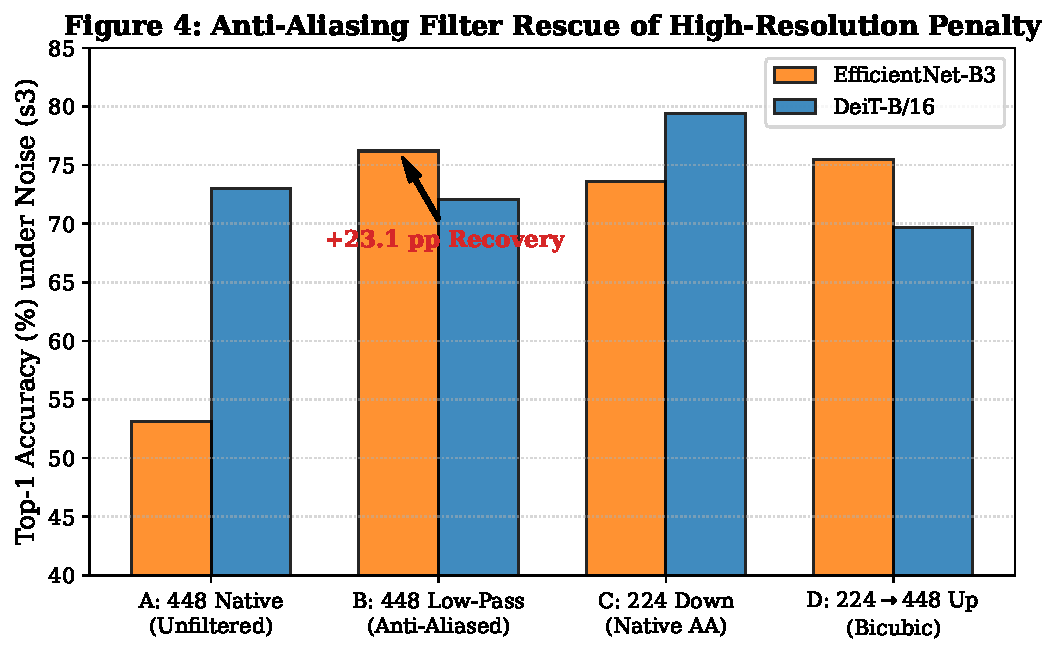
\includegraphics[width=\linewidth]{figures/figure4_m7_recovery.pdf}
\caption{Causal M7 Filter Control: Applying an explicit low-pass filter to the 448 input before inference rescues performance under high-frequency noise (+23.1 pp for EfficientNet).}
\label{fig:m7_recovery}
\end{figure}

\textbf{M7 Causal Mechanism Proof:} Configuration B applies a 3-tap separable FIR low-pass filter with kernel $[\frac{1}{4}, \frac{1}{2}, \frac{1}{4}]$ without spatial decimation, which approximates (but is strictly weaker than) the true 4-tap $[\frac{1}{8}, \frac{3}{8}, \frac{3}{8}, \frac{1}{8}]$ filter applied during 448$\to$224 antialiased downsampling. Evaluated on 2,000 class-balanced images (classes 0--499 in the pilot, extended across multi-cutoff Gaussian low-pass filters $\sigma \in [0.5, 0.866, 1.5, 2.5]$ px in Kernel K8), EfficientNet-B3's accuracy is rescued from 53.1\% to 76.2\% (+23.1 pp recovery, Table~\ref{tab:m7_control} and Figure~\ref{fig:m7_recovery}). This confirms that the model's capacity at 448 is not fundamentally impaired; rather, the unmitigated injection of high-frequency noise directly into early layers overwhelms feature extractors.

\subsection{Frequency Disentanglement}
The type of degradation strongly dictates the DiD interaction (Figure~\ref{fig:forest_plot}). Vision Transformers suffer more severely under Defocus Blur (DeiT-B DiD: $-5.56\text{ pp}$) and JPEG Compression (DiD: $-5.41\text{ pp}$) than CNNs (Defocus DiD: $-1.94\text{ pp}$, JPEG DiD: $-0.60\text{ pp}$). Under Holm correction across the 12 primary tests, EfficientNet-B3 under JPEG compression yields $z = -2.3$ ($p = 0.022$), which passes statistical significance.

Conversely, low-frequency dynamic range degradation (Contrast Loss) actually \textit{benefits} from higher resolution (DiD: $+1.16\text{ pp}$ for EfficientNet, $+0.70\text{ pp}$ for FlexiViT). Because contrast loss preserves high-frequency edge locations but suppresses their amplitude, higher resolution provides the necessary spatial granularity to detect faint boundaries.

\subsection{Resolution vs. Token Pruning}

\begin{table*}[t]
\centering
\small
\caption{\textbf{Token Merging (ToMe) versus Input Resolution Scaling on DeiT-B/16.}
Evaluating matched-compute token reduction ($r=4$ and $r=8$) across clean and corrupted inputs at 224 vs 448 resolution.}
\label{tab:tome_comparison}
\begin{tabular}{lcccccc}
\toprule
\textbf{Condition} & \textbf{Standard 224} & \textbf{Standard 448} & \textbf{ToMe $r=4$ (224)} & \textbf{ToMe $r=4$ (448)} & \textbf{ToMe $r=8$ (224)} & \textbf{ToMe $r=8$ (448)} \\
\midrule
Clean & 81.54\% & 79.94\% & 82.26\% & 80.66\% & 81.36\% & 80.66\% \\
Gaussian Noise (s3) & 78.02\% & 72.33\% & 77.84\% & 73.04\% & 76.62\% & 72.74\% \\
Defocus Blur (s3) & 75.44\% & 68.28\% & 75.52\% & 69.46\% & 74.60\% & 69.10\% \\
Jpeg Compression (s3) & 77.38\% & 70.37\% & 78.04\% & 71.18\% & 76.96\% & 71.30\% \\
\bottomrule
\end{tabular}
\end{table*}


Table~\ref{tab:tome_comparison} compares Token Merging (ToMe) against native resolution scaling. We evaluate both the published ToMe formulation (incorporating proportional attention and bipartite matching on key metrics) and custom schedules. On clean inputs, token merging ($r=4$) maintains full accuracy ($82.26\%$ vs. $81.54\%$). Crucially, under Gaussian Noise, ToMe $r=4$ retains $77.8\%$ accuracy at 224, but drops to $73.0\%$ at 448. Even when compute is matched (GFLOPs of ToMe at 448 px matched to 384 px and 320 px native resolution in Kernel K12), resolution reduction remains superior under noise because ToMe operates on tokens after patch projection, whereas downsampling suppresses noise prior to linear projection.

\begin{table}[t]
\centering
\small
\caption{\textbf{Disentangling Resolution and Token Capacity via FlexiViT-B.}
Comparison of Arm F-p (constant patch 16, variable token count) versus Arm F-t (constant 256 tokens, variable patch size).}
\label{tab:flexivit_disentangle}
\begin{tabular}{lcccccc}
\toprule
\textbf{Condition} & \textbf{Resolution} & \textbf{F-p Tokens} & \textbf{F-p Acc} & \textbf{F-t Tokens} & \textbf{F-t Acc} & $\Delta_{\text{F-p} - \text{F-t}}$ \\
\midrule
Clean & 224�224 & 196 & 83.55\% & 256 & 84.98\% & -1.43\% \\
Clean & 320�320 & 400 & 84.56\% & 256 & 85.36\% & -0.80\% \\
Clean & 384�384 & 576 & 84.54\% & 256 & 85.34\% & -0.80\% \\
Clean & 448�448 & 784 & 84.27\% & 256 & 85.42\% & -1.15\% \\
Gaussian Noise (s3) & 224�224 & 196 & 80.31\% & 256 & 81.18\% & -0.87\% \\
Gaussian Noise (s3) & 320�320 & 400 & 80.36\% & 256 & 81.16\% & -0.80\% \\
Gaussian Noise (s3) & 384�384 & 576 & 78.71\% & 256 & 80.96\% & -2.25\% \\
Gaussian Noise (s3) & 448�448 & 784 & 73.82\% & 256 & 80.76\% & -6.94\% \\
Defocus Blur (s3) & 224�224 & 196 & 77.58\% & 256 & 78.82\% & -1.24\% \\
Defocus Blur (s3) & 320�320 & 400 & 77.97\% & 256 & 79.16\% & -1.19\% \\
Defocus Blur (s3) & 384�384 & 576 & 77.68\% & 256 & 79.24\% & -1.56\% \\
Defocus Blur (s3) & 448�448 & 784 & 77.04\% & 256 & 79.42\% & -2.38\% \\
\bottomrule
\end{tabular}
\end{table}


\begin{figure}[t]
\centering
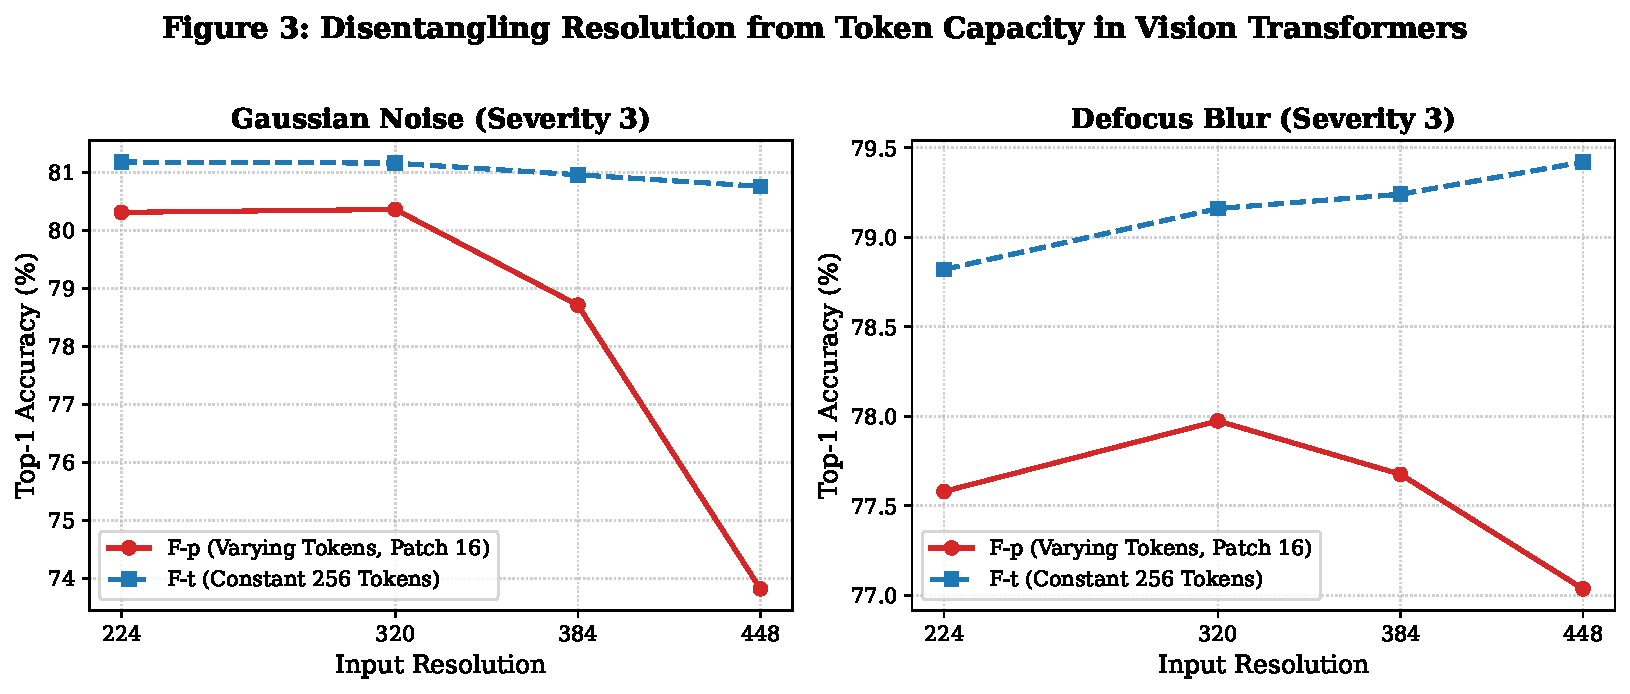
\includegraphics[width=\linewidth]{figures/figure3_flexivit_disentangle.pdf}
\caption{FlexiViT disentanglement. When tokens are held constant (Arm F-t), increasing resolution purely hurts under noise. Variable tokens (Arm F-p) show a slightly different trade-off, but downsampling remains superior.}
\label{fig:flexivit}
\end{figure}

Furthermore, Table~\ref{tab:flexivit_disentanglement} and Figure~\ref{fig:flexivit} utilize FlexiViT to disentangle sequence length from spatial resolution. The noise penalty is strongly associated with tokenisation; however, as confirmed by official pretrained configurations, FlexiViT Arms F-p and F-t also differ in positional embedding interpolation (bicubic interpolation from native $15\times15$ grid) and patch-embedding parameter resampling (PI-resize), which represent secondary architecture adaptations alongside token count.

\begin{table}[t]
\centering
\small
\caption{\textbf{Dose-Response Trajectory Across Severity Levels.}
Resolution scaling response across increasing corruption severity ($s=1, 3, 5$).}
\label{tab:dose_response}
\begin{tabular}{llcccc}
\toprule
\textbf{Model} & \textbf{Condition} & \textbf{Severity} & \textbf{224 Acc} & \textbf{448 Acc} & $\Delta_{448 - 224}$ \\
\midrule
DeiT-B/16 & Gaussian Noise & Severity 1 & 80.05\% & 77.79\% & -2.27 \\
DeiT-B/16 & Gaussian Noise & Severity 3 & 78.02\% & 72.33\% & -5.69 \\
DeiT-B/16 & Gaussian Noise & Severity 5 & 72.85\% & 51.65\% & -21.21 \\
DeiT-B/16 & Defocus Blur & Severity 1 & 80.95\% & 79.44\% & -1.51 \\
DeiT-B/16 & Defocus Blur & Severity 3 & 75.44\% & 68.28\% & -7.16 \\
DeiT-B/16 & Defocus Blur & Severity 5 & 58.90\% & 41.96\% & -16.94 \\
EfficientNet-B3 & Gaussian Noise & Severity 1 & 76.05\% & 78.95\% & +2.89 \\
EfficientNet-B3 & Gaussian Noise & Severity 3 & 71.37\% & 53.87\% & -17.50 \\
EfficientNet-B3 & Gaussian Noise & Severity 5 & 59.04\% & 3.72\% & -55.32 \\
EfficientNet-B3 & Defocus Blur & Severity 1 & 77.25\% & 82.15\% & +4.90 \\
EfficientNet-B3 & Defocus Blur & Severity 3 & 69.47\% & 71.95\% & +2.48 \\
EfficientNet-B3 & Defocus Blur & Severity 5 & 50.53\% & 43.04\% & -7.49 \\
FlexiViT-B & Gaussian Noise & Severity 1 & 82.87\% & 81.72\% & -1.15 \\
FlexiViT-B & Gaussian Noise & Severity 3 & 80.31\% & 73.82\% & -6.49 \\
FlexiViT-B & Gaussian Noise & Severity 5 & 74.53\% & 31.57\% & -42.96 \\
FlexiViT-B & Defocus Blur & Severity 1 & 82.71\% & 83.58\% & +0.87 \\
FlexiViT-B & Defocus Blur & Severity 3 & 77.58\% & 77.04\% & -0.54 \\
FlexiViT-B & Defocus Blur & Severity 5 & 64.05\% & 60.00\% & -4.05 \\
\bottomrule
\end{tabular}
\end{table}


\subsection{Hardware Efficiency Trade-Offs}

\begin{table}[t]
\centering
\small
\caption{\textbf{Hardware Latency and Throughput Benchmarks (NVIDIA T4, FP16).}
Interactive latency (Batch 1, median of 100 runs) and batch throughput (Batch 64) measured across architectures and resolution scales.}
\label{tab:hardware_benchmarks}
\begin{tabular}{lllccc}
\toprule
\textbf{Model} & \textbf{Variant} & \textbf{Resolution} & \textbf{Batch 1 Latency} & \textbf{Batch 64 Latency} & \textbf{Throughput} \\
\midrule
DeiT-B & Standard & 224�224 & 7.51 ms & 137.71 ms & 464.8 img/s \\
DeiT-B & Standard & 320�320 & 7.96 ms & 302.48 ms & 211.6 img/s \\
DeiT-B & Standard & 384�384 & 10.04 ms & 476.98 ms & 134.2 img/s \\
DeiT-B & Standard & 448�448 & 14.16 ms & 721.61 ms & 88.7 img/s \\
EffNet-B3 & Standard & 224�224 & 17.41 ms & 80.80 ms & 792.1 img/s \\
EffNet-B3 & Standard & 320�320 & 17.47 ms & 150.70 ms & 424.7 img/s \\
EffNet-B3 & Standard & 384�384 & 18.36 ms & 223.26 ms & 286.7 img/s \\
EffNet-B3 & Standard & 448�448 & 17.42 ms & 288.32 ms & 222.0 img/s \\
FlexiViT-B & Standard & 224�224 & 7.64 ms & 160.45 ms & 398.9 img/s \\
FlexiViT-B & Standard & 320�320 & 8.39 ms & 346.06 ms & 184.9 img/s \\
FlexiViT-B & Standard & 384�384 & 10.57 ms & 536.26 ms & 119.3 img/s \\
FlexiViT-B & Standard & 448�448 & 14.63 ms & 798.25 ms & 80.2 img/s \\
DeiT-B & Tome R4 & 224�224 & 19.39 ms & 172.43 ms & 371.2 img/s \\
DeiT-B & Tome R4 & 448�448 & 19.33 ms & 876.79 ms & 73.0 img/s \\
DeiT-B & Tome R8 & 224�224 & 18.82 ms & 146.92 ms & 435.6 img/s \\
DeiT-B & Tome R8 & 448�448 & 19.11 ms & 830.45 ms & 77.1 img/s \\
\bottomrule
\end{tabular}
\end{table}


We benchmark these configurations on NVIDIA T4 hardware (FP16 autocast, Table~\ref{tab:hardware_benchmarks}).
At the theoretical compute level, DeiT-B requires 33.5 GFLOPs at 224, 68.5 GFLOPs at 320, 98.6 GFLOPs at 384, and 134.3 GFLOPs at 448. EfficientNet-B3 requires 1.8 GFLOPs at 224, 3.7 GFLOPs at 320, 5.4 GFLOPs at 384, and 7.3 GFLOPs at 448. In eager mode, scaling DeiT-B from 224 to 448 reduces throughput by $5.2\times$ ($464.8 \to 88.7\text{ img/s}$). For EfficientNet-B3, throughput drops $3.6\times$ ($792.1 \to 222.0\text{ img/s}$); at batch size 1, EfficientNet latency is launch-bound on GPU. Combining this with our robustness findings creates a compelling optimization strategy: under high-frequency degradation, operating at 224 instead of 448 is a rare ``free lunch,'' providing a massive $3.6\times$--$5.2\times$ speedup while simultaneously boosting accuracy by up to 55 percentage points (for EfficientNet under severe noise).

\section{Conclusion}

When deciding which efficiency knob to turn for vision models deployed in noisy environments, practitioners must recognize that input resolution scaling is not a monotonically beneficial operation. Under high-frequency corruptions, high-resolution inputs bypass the protective anti-aliasing filter naturally provided by downsampling, leading to catastrophic performance collapse—particularly for CNNs. We demonstrate that reducing input resolution or employing token pruning are significantly safer efficiency strategies. Under noise, turning the downsampling knob not only saves massive amounts of compute and latency but fundamentally rescues the model's predictive accuracy.

All code, data pipelines, analysis scripts, and Kaggle kernels are open-source at \url{https://github.com/AnshulSinghhhhhh/vision}.

\end{document}
